% !TEX TS-program = XeLaTeX
% !TEX encoding = UTF-8 Unicode

\chapter{系统设计}

\label{chap07}

\defaultfont

\section{系统整体模块设计}

系统整体模块设计如图\ref{system-wbs}所示,总体可以分为学生模块,教师模块,管理员模块。在学生模块中可以进一步将功能细分为论文上传功能,论文下载功能,成绩查看功能,回复评论功能,论文更新功能。教师模块可以进一步分为查看所管理的学生论文信息功能,论文下载功能,论文评论功能,论文添加问题标签功能,论文评分功能。管理模块可以进一步分为系统管理和论文管理,系统管理可以进一步分为用户管理,上传通道管理,论文管理可以进一步分为评审情况统计,教师评审情况统计。

\begin{figure}[h]
    \centering
    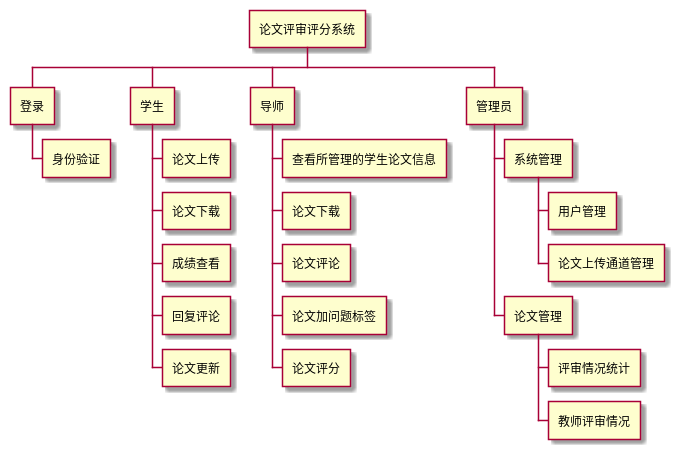
\includegraphics[scale = 0.6]{out/uml/WBS/系统WBS/系统WBS.png}
    \caption{\song\wuhao 系统整体模块}
    \label{system-wbs}
\end{figure}

\section{系统架构设计}

如图\ref{system-frame-deployment}所示,本系统采用的时前后端分离架构,系统前端使用vue,Element Plus UI,axios,vuex,vue-router,系统后端使用了Spring Boot,同时配置Tomcat,Spring Security,Spring Data JPA,系统的持久化选择Hibernate和MySQL。

前后端分离架构优势:
\begin{enumerate}
    \item 系统的可伸缩性。\\由于将代码分成前端和后端两部分,可以不用考虑对方进行对立优化,只要保证数据接口不改变,那么双方的交互就不会出现问题。
    \item 减少资源传递。\\在以往的非前后端分离项目中,服务器要做的工作有解析请求,从数据库中检索相关数据并处理数据,然后结合HTML模板并将其发送给浏览器。而在前后端分离的系统中,服务器并不需要处理HTML,之需要将处理好的数据作为response(一般是JSON对象)返还给前端,而前端根据数据进行展示,这个过程减少了服务器的任务,因此降低了服务器的压力,并且用户体验更好,因为整个页面不会随着每个请求而更新。
    \item 更容易升级。\\升级架构是一件痛苦的事情。前后端分类可以更好地进行升级和调试,通过查看接口地返回数据地正确与否就可以判断是前端的问题还是后端的问题,这在系统升级的过程中可以加速问题的排查。
    \item 更容易切换框架。\\现如今技术的的变化很快,不仅现在使用的框架更新频率很高,并且新的更好的框架也层出不穷。在使用前后端分离架构的情况下,前后端并不关心对方使用的是什么框架,只需要规定好接口并且保证在切换框架的过程同接口不会改变。比如前端从Vue转变为Angular,这个变化后端并不会有感知。
    \item 更快地部署。\\由于前端开发人员和后端开发人员并不需要太多地相互依赖(只有在定义接口地时候需要双方协商),所以前后端可以独立进行测试和部署而无需等待对方任务的完成。
    \item 整合的API。\\当前端需要多平台部署时,例如Web端,移动端,在开发应用的过程中,不需要为各自的编写不同的后台,两者可以使用相同的后台,即使用相同的API,这无疑减小了不必要的、重复的代码编写。而且在使用相同的API的情况下可以保证各个平台的数据的一致性,以及后台升级时,各个平台同时获得更新。
    \item 模块化。\\如果您的前端与后端分离,那么在一个模块上工作而不影响另一个模块就变得更容易了。模块化还使两个团队或两个人同时在前端和后端工作变得更容易,而不必担心覆盖或搞乱其他人的工作。他们也可以用不同的节奏工作。
\end{enumerate}

\begin{figure}[h]
    \centering
    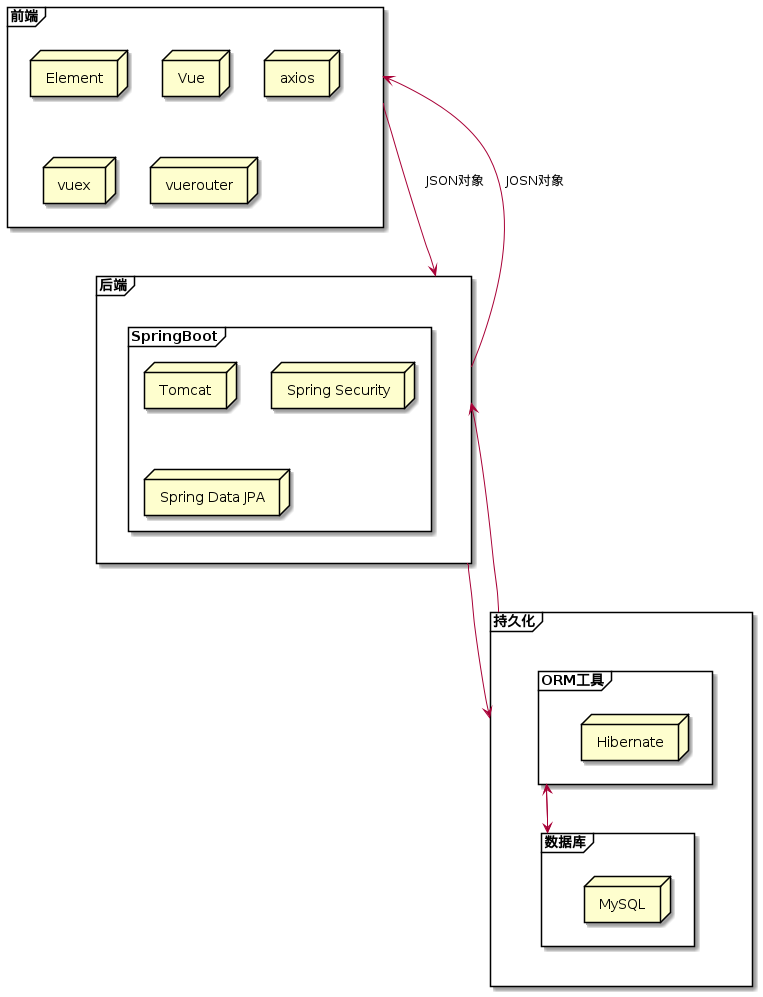
\includegraphics[scale = 0.5]{out/uml/部署图/系统架构/系统架构.png}
    \caption{\song\wuhao 系统架构设计}
    \label{system-frame-deployment}
\end{figure}

\section{数据库设计}
\subsection{概念结构设计}
\subsection{逻辑结构设计}
\subsection{物理结构设计}

